\documentclass[10pt,border=0pt]{standalone}
\usepackage[T1]{fontenc}
\usepackage[utf8]{inputenc}
\usepackage{pgfplots}
\pgfplotsset{compat=1.18}
\usepgfplotslibrary{groupplots}
\definecolor{SGblue}{HTML}{0072B2}
\definecolor{arPLSvermillion}{HTML}{D55E00}
\renewcommand{\familydefault}{\rmdefault}
\begin{document}
\begin{minipage}{181.86mm}
\vspace*{6pt}\noindent\hspace*{3pt}
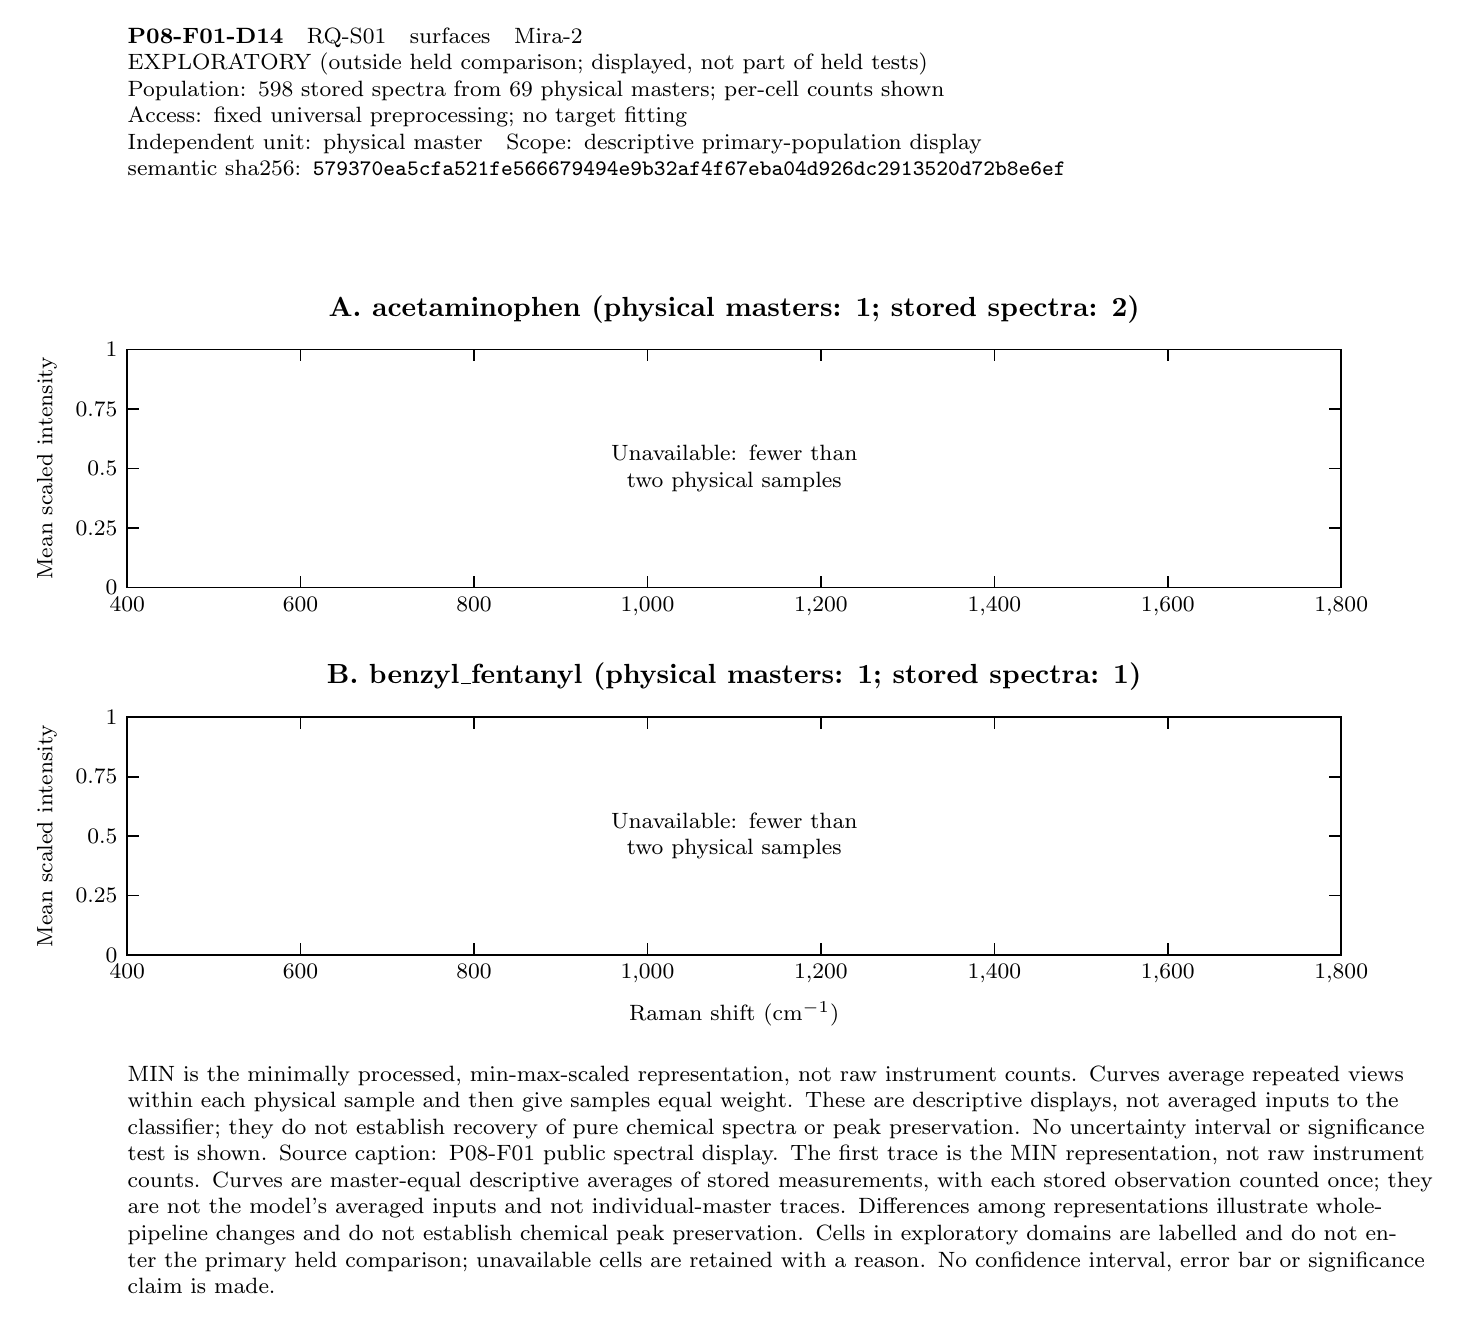
\begin{tikzpicture}
\begin{groupplot}[
  group style={group size=1 by 2, vertical sep=1.65cm},
  width=17cm, height=4.6cm,
  xmin=400, xmax=1800, ymin=0, ymax=1,
  xtick={400,600,800,1000,1200,1400,1600,1800},
  ytick={0,0.25,0.5,0.75,1},
  tick label style={font=\fontsize{8}{9.6}\selectfont, text=black},
  label style={font=\fontsize{8}{9.6}\selectfont, text=black},
  title style={font=\bfseries\fontsize{10}{12}\selectfont, text=black, align=center},
  axis line style={black, line width=0.6pt},
  tick style={black, line width=0.6pt},
  ylabel={Mean scaled intensity},
]
\nextgroupplot[title={A. acetaminophen (physical masters: 1; stored spectra: 2)}]
\node[anchor=center, text=black, font=\fontsize{8}{9.6}\selectfont, text width=5.5cm, align=center] at (axis description cs:0.5,0.5) {Unavailable: fewer than two physical samples};
\nextgroupplot[title={B. benzyl\_fentanyl (physical masters: 1; stored spectra: 1)}, xlabel={Raman shift (cm$^{-1}$)}]
\node[anchor=center, text=black, font=\fontsize{8}{9.6}\selectfont, text width=5.5cm, align=center] at (axis description cs:0.5,0.5) {Unavailable: fewer than two physical samples};
\end{groupplot}
\node[anchor=south west, align=left, inner sep=0pt, font=\fontsize{8}{9.6}\selectfont, text=black, text width=166mm] at ([yshift=22mm]group c1r1.north west) {\textbf{P08-F01-D14}\quad RQ-S01\quad surfaces\quad Mira-2\\EXPLORATORY (outside held comparison; displayed, not part of held tests)\\Population: 598 stored spectra from 69 physical masters; per-cell counts shown\\Access: fixed universal preprocessing; no target fitting\\Independent unit: physical master\quad Scope: descriptive primary-population display\\semantic sha256: {\fontsize{8}{9.6}\selectfont\texttt{579370ea5cfa521fe566679494e9b32af4f67eba04d926dc2913520d72b8e6ef}}};
\node[anchor=north west, align=left, inner sep=0pt, font=\fontsize{8}{9.6}\selectfont, text=black, text width=166mm] at ([yshift=-14mm]group c1r2.south west) {MIN is the minimally processed, min-max-scaled representation, not raw instrument counts. Curves average repeated views within each physical sample and then give samples equal weight. These are descriptive displays, not averaged inputs to the classifier; they do not establish recovery of pure chemical spectra or peak preservation. No uncertainty interval or significance test is shown. Source caption: P08-F01 public spectral display. The first trace is the MIN representation, not raw instrument counts. Curves are master-equal descriptive averages of stored measurements, with each stored observation counted once; they are not the model's averaged inputs and not individual-master traces. Differences among representations illustrate whole-pipeline changes and do not establish chemical peak preservation. Cells in exploratory domains are labelled and do not enter the primary held comparison; unavailable cells are retained with a reason. No confidence interval, error bar or significance claim is made.};
\end{tikzpicture}\par\vspace*{6pt}
\end{minipage}
\end{document}
